% ICASSP 2027 manuscript: official SPS conference template (spconf.sty / IEEEbib.bst).
\documentclass{article}
\usepackage{spconf,amsmath,amssymb,graphicx,tikz,hyperref,flushend}
\usetikzlibrary{arrows.meta,calc,positioning}

\title{Beyond Reference Matching: Specification-Based Correctness\\
Evaluation for DSP Implementations}

\name{Xianghui Meng$^{1}$ and Jionghao Lin$^{1,2,\ast}$}
\address{$^{1}$The University of Hong Kong \\
$^{2}$Carnegie Mellon University \\
\texttt{margretmeng1020@gmail.com} \\
$^{\ast}$Corresponding author: \texttt{jionghao@hku.hk}}

\begin{document}
\maketitle

\begin{abstract}
A reference implementation is commonly used as the correctness target
for DSP implementations.
That comparison is exact for a unique map, but a magnitude mask
defines a feasible set, not one coefficient vector.
We score a candidate by specification-set membership ($S_t=1$ if it
meets a frozen contract) and compare coefficient and spec-band
response agreement to one canonical design.
On 20 non-unique mask instances, reference matching rejects
$374/416$ constructed-valid implementations
($\mathrm{FRR}_{\mathrm{ref}}=0.899$; $0.927$ on tight masks).
On eight singleton identities, $\mathrm{FRR}_{\mathrm{ref}}=0$.
Against the same constructed labels, the coefficient oracle has
$\mathrm{FRR}=0.899$ and $\mathrm{FAR}=0$, and spec-band similarity
has $\mathrm{FRR}=0.067$ and $\mathrm{FAR}=0$; membership
$\mathrm{FRR}=\mathrm{FAR}=0$ restates the admission rule.
The same $S_t=1$, $R_{t,r}=0$ event appears among existing generated
implementations.
On these non-unique specifications, reference agreement is a
realization diagnostic.
Our code is available at:
\url{https://github.com/XianghuiMeng-1020/dsp-semantic-correctness}.
\end{abstract}

\begin{keywords}
Filter design, specification testing, correctness evaluation, FIR, IIR
\end{keywords}

\section{Introduction}
\label{sec:intro}

Evaluating a DSP implementation against a trusted reference is natural
when the specification is a unique map: one integer delay, one declared
Fourier convention, one alias-fold period.
In those cases, coefficient or output agreement with the reference
\emph{is} correctness.

Classical filter design is different.
A magnitude mask with a free transition defines a
\emph{feasible set} of realizations, not a unique impulse
response~\cite{oppenheim2010dsp,proakis2007dsp,mitra2011dsp,rabiner1975theory}.
Windowed designs~\cite{kaiser1974window,harris1978windows},
frequency sampling~\cite{rabiner1970freqsamp},
equiripple Parks--McClellan approximation~\cite{parks1972chebyshev,mcclellan1973computer,rabiner1975fir},
and IIR Butterworth or elliptic sections~\cite{butterworth1930,constantinides1970,jackson1996filters,antoniou2006filters}
can all meet the same passband, stopband, and stability bounds while
remaining far apart as coefficient vectors.
A canonical library call---Hamming \texttt{firwin}, or a Butterworth
section~\cite{virtanen2020scipy}---is one occupant of that set.

Therefore a valid reference cannot, by itself, define correctness over
the whole set.
Matching that reference asks whether a candidate is the
\emph{same realization}.
It does not ask whether the candidate meets the contract that
justified the reference.

This paper treats that distinction as an evaluation problem for
generated DSP implementations~\cite{chen2021codex,liu2023evalplus},
not as a model leaderboard and not as a new design algorithm.
The object of study is the scoring rule, not model quality.

Formally, reference agreement $R_{t,r}(h)=1$ asks whether $h$ matches
a particular realization $h_r$.
Specification membership $S_t(h)=1$ asks whether $h$ meets the
frozen contract.
When the feasible set $\mathcal{V}_t=\{h:S_t(h)=1\}$ contains more
than one realization, these questions diverge:
$R_{t,r}$ is a realization diagnostic, and $S_t$ is the correctness
criterion used below.
When the specification is effectively a singleton under the
declared scoring tolerance, they should agree.

Related work falls in three clusters.
Filter-approximation texts treat the mask as a feasible-set
problem~\cite{oppenheim2010dsp,rabiner1975fir,herrmann1973linear}.
DSP algorithm tests may use a golden
reference~\cite{huuhtanen2015dsp}.
A standard generated-code protocol uses unique-output unit
tests~\cite{liu2023evalplus}; that protocol does not score a
non-unique DSP mask.
We do not survey model families.

We make three contributions.
(i)~We distinguish realization agreement from specification-set
membership as scoring rules for DSP implementations.
(ii)~We construct a singleton suite and a non-unique magnitude-mask
suite with frozen valid and invalid labels, independent of reference
distance.
(iii)~We measure the evaluation consequence: reference false rejection
is high on the constructed non-unique suite, zero on the singleton
suite, and the same $S_t=1$,~$R_{t,r}=0$ event appears among
existing generated implementations.

\section{Problem formulation}
\label{sec:form}

A design task $t$ asks for an implementation $h$ (FIR taps, or an IIR
pair $(b,a)$).
A frozen specification predicate returns $S_t(h)\in\{0,1\}$.
The feasible set is
\begin{equation}
\mathcal{V}_t=\{h:S_t(h)=1\}.
\label{eq:vt}
\end{equation}
A canonical reference $h_r$ is one occupant, $h_r\in\mathcal{V}_t$,
and nothing stronger: it is a convenient valid realization, not the
definition of $t$.

The task is treated as a \emph{singleton} when the declared map is
unique up to the scoring tolerance (unique lag, unique DFT convention,
unique alias map, unique impulse).
It is \emph{non-unique} when more than one realization meets $S_t$.
The non-unique family studied here is a classical magnitude mask:
constrained pass and stop bands on $\lvert H(f)\rvert$, a free
transition, and, for IIR, a pole-radius stability bound.
Linear phase is not required.

\section{Specification-based evaluation}
\label{sec:method}

Write $\tilde h$ for the coefficient vector of $h$, or the
concatenation $(b,a)$, truncated to the shorter length when orders
differ.
Oracle~A (reference coefficients) is
\begin{equation}
R_{t,r}(h)
=\mathbf{1}\!\left[
\frac{\lVert \tilde h-\tilde h_r\rVert_2}{\lVert\tilde h_r\rVert_2}
\le\tau_R\right],
\label{eq:r}
\end{equation}
with frozen $\tau_R=0.05$.
$R_{t,r}(h)=1$ asks whether $h$ is the same realization as $h_r$.

Oracle~B (response similarity) accepts $h$ when the
$\lvert H\rvert$ RMSE on constrained bands versus $h_r$ does not
exceed the maximum same-order library-pair RMSE on that instance,
plus $10^{-8}$.
Oracle~B is a DSP-native comparison to \emph{one} element of
$\mathcal{V}_t$.
It is not a gold standard for correctness.

Oracle~C implements the same predicate $S_t$ used to admit
constructed labels; it is the membership checker, not an external
labeler.
On each constrained band $[f_0,f_1]$ with bounds $[\ell,u]$, a
$4096$-point \texttt{freqz} residual records the worst normalized
excursion of $\lvert H\rvert$ outside $[\ell,u]$.
FIR contracts pass at residual $\le 10^{-6}$; IIR contracts also
require every pole radius $<0.999$ and pass at residual
$\le 10^{-3}$.
Neither floor was fit to generated residuals.
The checker does not load $h_r$, does not compute coefficient
distance, and does not call Oracle~A or~B.
A tone-envelope consistency check $T$ reads the same mask and is not
used as gold for FAR/FRR.

Fig.~\ref{fig:concept} states the geometry: the $\tau_R$-ball around
$h_r$ is a realization neighborhood; $\mathcal{V}_t$ is the contract.

\begin{figure*}[t]
\centering
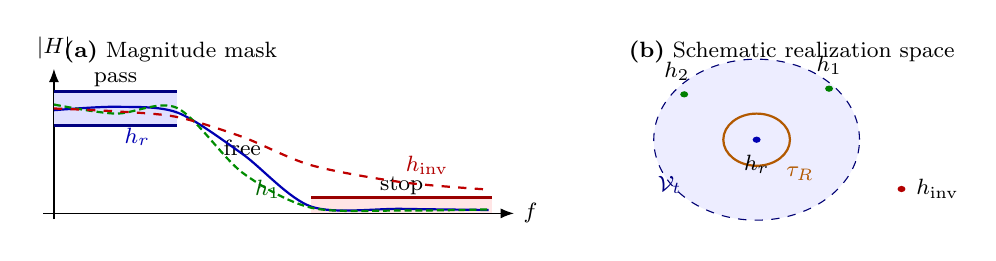
\begin{tikzpicture}[x=0.92cm,y=0.72cm,font=\footnotesize]
  % ---- left: mask ----
  \draw[-{Latex}] (-0.15,0) -- (6.35,0) node[right] {$f$};
  \draw[-{Latex}] (0,-0.1) -- (0,2.55) node[above] {$\lvert H\rvert$};
  \fill[blue!12] (0,1.55) rectangle (1.7,2.15);
  \fill[red!10] (3.55,0) rectangle (6.05,0.28);
  \draw[blue!50!black,thick] (0,1.55) -- (1.7,1.55);
  \draw[blue!50!black,thick] (0,2.15) -- (1.7,2.15);
  \draw[red!60!black,thick] (3.55,0.28) -- (6.05,0.28);
  \node at (0.85,2.35) {pass};
  \node at (2.6,1.15) {free};
  \node at (4.8,0.48) {stop};
  \draw[blue!70!black,thick] plot[smooth] coordinates {(0,1.82) (0.85,1.88) (1.7,1.78) (2.6,1.05) (3.55,0.12) (4.8,0.08) (6.0,0.06)};
  \draw[green!55!black,thick,dash pattern=on 2.5pt off 1.4pt] plot[smooth] coordinates {(0,1.92) (0.85,1.76) (1.7,1.86) (2.6,0.72) (3.55,0.10) (4.8,0.05) (6.0,0.07)};
  \draw[red!75!black,thick,dashed] plot[smooth] coordinates {(0,1.85) (0.85,1.80) (1.7,1.70) (2.6,1.35) (3.55,0.85) (4.8,0.55) (6.0,0.42)};
  \node[blue!70!black] at (1.15,1.35) {$h_r$};
  \node[green!40!black] at (2.95,0.42) {$h_1$};
  \node[red!70!black] at (5.15,0.85) {$h_{\mathrm{inv}}$};
  \node[font=\footnotesize,anchor=west] at (0,2.85) {\textbf{(a)} Magnitude mask};
  % ---- right: realization ----
  \begin{scope}[shift={(8.15,0.15)}]
    \fill[blue!7] (1.55,1.15) circle (1.42);
    \draw[blue!45!black,dashed] (1.55,1.15) circle (1.42);
    \draw[orange!70!black,thick] (1.55,1.15) circle (0.46);
    \fill[blue!70!black] (1.55,1.15) circle (0.055);
    \node[below] at (1.55,1.05) {$h_r$};
    \fill[green!50!black] (2.55,2.05) circle (0.055);
    \node[above] at (2.55,2.12) {$h_1$};
    \fill[green!50!black] (0.55,1.95) circle (0.055);
    \node[above] at (0.45,2.02) {$h_2$};
    \fill[red!70!black] (3.55,0.28) circle (0.055);
    \node[right] at (3.62,0.28) {$h_{\mathrm{inv}}$};
    \node[orange!70!black] at (2.15,0.55) {$\tau_R$};
    \node[blue!50!black] at (0.35,0.35) {$\mathcal{V}_t$};
    \node[font=\footnotesize,anchor=west] at (-0.35,2.70) {\textbf{(b)} Schematic realization space};
  \end{scope}
\end{tikzpicture}
\caption{Same contract, two spaces.
(a)~Frequency-domain magnitude mask.
(b)~Schematic realization/coefficient space: the $\tau_R$-ball is
proximity to one valid $h_r$; the $\mathcal{V}_t$ region is
schematic and is not a Euclidean ball in the same metric as
$\tau_R$.
Occupants $h_1,h_2$ meet the mask but lie outside the reference
ball; $h_{\mathrm{inv}}$ violates the contract.}
\label{fig:concept}
\end{figure*}

\section{Experimental protocol}
\label{sec:protocol}

Two suites are scored (Table~\ref{tab:suite}).
Suite~S comprises eight singleton identities already used as
unique-map contracts (integer delay, circular and linear convolution
conventions, lag-$0$ energy, alias fold, frequency rescale, Nyquist
frequency, and $\delta[n-D]$).
Suite~N comprises $20$ specification instances from a common
magnitude-mask family: FIR low-pass, high-pass, band-pass, and
band-stop at $f_s=8$ and $16\,\mathrm{kHz}$, each at a loose and a
tight mask ($16$ FIR), plus IIR low-pass and high-pass at $8\,\mathrm{kHz}$
(loose/tight; $4$ IIR).
Loose $8\,\mathrm{kHz}$ prototypes reuse the previously frozen
pass/stop numbers.
Tight masks are derived mechanically (pass ripple and stop ceiling
$\times 1/5$; stop edge moved halfway toward the facing pass).
Sixteen-kilohertz edges are the $8\,\mathrm{kHz}$ edges $\times 2$.
Canonical $h_r$ is the shortest-odd Hamming \texttt{firwin} (FIR) or
the lowest-order \texttt{butter} (IIR) that meets $S_t$.

Suite~N valids are constructed from three sources: classical library
designers (\texttt{firwin}, \texttt{firwin2}, \texttt{remez},
\texttt{firls}, Kaiser \texttt{firwin}; \texttt{butter},
\texttt{cheby1}, \texttt{cheby2}, \texttt{ellip}); first-principles FIR
windowed-sinc and frequency sampling (numpy only; SciPy design APIs
forbidden)~\cite{kaiser1974window,rabiner1970freqsamp}; and
random-valid search over odd length, window or Remez weights, and
cutoffs in the free transition (IIR: prototype and order).
Admission is $S_t(h)=1$ only.
Distance to $h_r$ is measured after admission.
Occupants that met $S_t$ and lay near $h_r$ were retained.
The random-valid search does not maximize coefficient distance,
response RMSE, or disagreement with $h_r$.
Near-duplicates are removed
($d_{\mathrm{coeff}}\le 0.01$ and full-grid $\lvert H\rvert$ RMSE
$\le 10^{-3}$); deduplication does not maximize distance.
The kept set has $416$ valids ($92$ library, $24$ first-principles,
$300$ random-valid).

Invalids are $144$ mechanism-based contract violations (band swap,
cutoff into a constrained band, insufficient order, unstable pole,
Nyquist coded as $1\,\mathrm{Hz}$, pass-gain collapse, wrong $f_s$,
and type mismatch), not a sample of naturally occurring errors.
A mutant is admitted only if $S_t=0$.
Labels were frozen before any oracle comparison.

Arm~G is a generated-code witness on the original four loose
$8\,\mathrm{kHz}$ masks only ($48$ planned draws; no new generations).
It is not pooled into the constructed $n$.
Constructed occupants score the oracles; Arm~G is only an
application witness.

Primary rates use constructed labels.
$\mathrm{FRR}_{\mathrm{ref}}$ is the fraction of valids with
$R_{t,r}=0$.
$\mathrm{FRR}_{\mathrm{ref}}^{\mathrm{any3}}$ rejects a valid only if
it is discordant with every available library occupant among
\texttt{firwin}/\texttt{remez}/\texttt{firls} (FIR) or the IIR library
set.
Oracles~A--C are scored as FRR/FAR against the same labels.
Suite~S uses the same definitions on identity outputs.

\begin{table}[t]
\caption{Study suites.
Arm~G is a witness on four original masks and is not added to the
constructed counts.}
\label{tab:suite}
\centering
\footnotesize
\setlength{\tabcolsep}{2.6pt}
\begin{tabular}{@{}lcccccc@{}}
\hline
Suite & Inst. & Spec.\ type & Uniq. & Valid & Invalid & Witness \\
\hline
S & $8$ & unique map & yes & $12$ & $16$ & --- \\
N & $20$ & mag.\ mask & no & $416$ & $144$ & Arm G, $4$ \\
\hline
\end{tabular}
\end{table}

\section{Results}
\label{sec:results}

\noindent\textbf{RQ1 --- Reference false rejection.}
On Suite~S, $\mathrm{FRR}_{\mathrm{ref}}=0/12$.
On Suite~N, reference matching rejects $374/416$ constructed-valid
implementations ($\mathrm{FRR}_{\mathrm{ref}}=0.899$;
Table~\ref{tab:frr}).
The rate is $302/340=0.888$ on FIR, $72/76=0.947$ on IIR,
$183/210=0.871$ on loose masks, and $191/206=0.927$ on tight masks.
Every one of the $20$ instances has at least one valid with
$S_t=1$ and $R_{t,r}=0$.
Best-of-three references still reject $346/416=0.832$.
These fractions describe disagreement inside constructed feasible
sets.
They are not rates over DSP implementations at large, and they are not
rates over generated code.

\begin{table}[t]
\caption{Reference rejection at $\tau_R=0.05$ on constructed-valid
occupants ($n$).
Task-level disagreement: instances with at least one constructed
valid that fails Oracle~A while meeting the contract.}
\label{tab:frr}
\centering
\footnotesize
\setlength{\tabcolsep}{3.0pt}
\begin{tabular}{@{}lcccc@{}}
\hline
Suite & $n$ & $\mathrm{FRR}_{\mathrm{ref}}$ & $\mathrm{FRR}_{\mathrm{ref}}^{\mathrm{any3}}$ & Task disag. \\
\hline
S & $12$ & $0/12=0$ & --- & --- \\
N all & $416$ & $374/416=0.899$ & $346/416=0.832$ & $20/20$ \\
N FIR & $340$ & $302/340=0.888$ & $274/340=0.806$ & --- \\
N IIR & $76$ & $72/76=0.947$ & $72/76=0.947$ & --- \\
N loose & $210$ & $183/210=0.871$ & $177/210=0.843$ & --- \\
N tight & $206$ & $191/206=0.927$ & $169/206=0.820$ & --- \\
\hline
\end{tabular}
\end{table}

\noindent\textbf{RQ2 --- Diversity of $\mathcal{V}_t$.}
Library, first-principles, and random-valid sources all contribute
occupants with $S_t=1$.
On every Suite~N instance the median min-length coefficient distance
to $h_r$ is at least $1.0$, while median spec-band $\lvert H\rvert$
RMSE stays on the order of $10^{-3}$ (FIR) to $10^{-2}$ (IIR);
full-grid RMSE is larger because the transition is unconstrained.
First-principles windowed-sinc and frequency-sampling designs enter
the same sets without calling a library designer, so multiplicity is
not an API artifact.
One concrete pattern: a same-order first-principles occupant can remain
inside the mask with spec-band RMSE $\sim 10^{-3}$ while
$d_{\mathrm{coeff}}>\tau_R$ versus Hamming \texttt{firwin}.
On the $67$ occupants whose order equals that of $h_r$,
$\mathrm{FRR}_{\mathrm{ref}}=25/67=0.373$, versus $0.899$ on the
unrestricted $416$ (Table~\ref{tab:ablate}).
Order variation contributes materially to coefficient disagreement.
A nonzero rate remains on this restricted subset: realization
equality is still not equivalent to contract membership.
All constructed FIR occupants in this set are Type~I, so a
linear-phase restriction is not a separate ablation here.
Varying $\tau_R\in\{0.01,0.05,0.10\}$ changes
$\mathrm{FRR}_{\mathrm{ref}}$ only from $0.933$ to $0.873$
(Table~\ref{tab:ablate}).

\begin{table}[t]
\caption{FRR/FAR on the contract-defined constructed universe
(N: $416$ valid, $144$ invalid; S: $12$ valid, $16$ invalid).
Oracle~C implements $S_t$, so its zeros check label consistency,
not independent validation.
The informative contrast is A and B on the same labels.
Oracle~B is undefined on Suite~S.}
\label{tab:oracle}
\centering
\footnotesize
\setlength{\tabcolsep}{3.2pt}
\begin{tabular}{@{}llcc@{}}
\hline
Suite & Oracle (rule) & FRR & FAR \\
\hline
N & A \ (coeff.\ vs.\ $h_r$, $\tau_R=0.05$) & $0.899$ & $0$ \\
N & B \ (band $\lvert H\rvert$ vs.\ $h_r$) & $0.067$ & $0$ \\
N & C \ (specification membership) & $0$ & $0$ \\
S & A \ (output vs.\ canonical) & $0$ & $0$ \\
S & C \ (specification membership) & $0$ & $0$ \\
\hline
\end{tabular}
\end{table}

\noindent\textbf{RQ3 --- Oracles versus constructed labels.}
Table~\ref{tab:oracle} compares A--C on the frozen contract-defined
universe.
Against those labels, Oracle~A has $\mathrm{FRR}=0.899$ and
$\mathrm{FAR}=0$: it never accepts a mutant, and it rejects most
valids.
Oracle~B has $\mathrm{FRR}=0.067$ and $\mathrm{FAR}=0$: most
constructed valids stay close to $h_r$ on the constrained bands,
so B rarely false-rejects even when the taps differ.
That agreement does not make B a membership test: it still scores
proximity to one realization.
Oracle~C has $\mathrm{FRR}=\mathrm{FAR}=0$ because it implements
the same $S_t$ used to write the labels; the row is
implementation consistency, not external validation of~C.
The informative comparison is how A and B reject subsets of the
same contract-valid set.
A asks realization identity.
B asks response proximity to one realization.
C asks contract satisfaction.

\noindent\textbf{RQ4 --- Singleton contrast.}
On Suite~S, Oracles~A and~C both have $\mathrm{FRR}=\mathrm{FAR}=0$.
The argument is conditional.
When the specification is a unique map, reference matching and
specification membership coincide, and reference matching is the
appropriate correctness test.
The Suite~N false-rejection rates are not a generic indictment of
reference comparison.

\noindent\textbf{RQ5 --- Generated-code witness.}
Among the existing eligible generated implementations on the
original four loose $8\,\mathrm{kHz}$ masks, nine satisfied the
frozen specification while failing reference agreement.
Such witnesses occurred on all four of those specification
instances.
This is an existence witness that the scoring mismatch is not
confined to constructed filters.
It is not a prevalence estimate and not a model comparison.

\section{Discussion}
\label{sec:disc}

\begin{table}[t]
\caption{Sensitivity of $\mathrm{FRR}_{\mathrm{ref}}$ on Suite~N
constructed valids.
The $\tau_R$ rows use all $416$ occupants.
The order-lock row uses only the $67$ occupants whose order equals
that of $h_r$.
Thresholds were not retuned after seeing outcomes.}
\label{tab:ablate}
\centering
\footnotesize
\setlength{\tabcolsep}{4.5pt}
\begin{tabular}{@{}lcc@{}}
\hline
Knob & $n$ & $\mathrm{FRR}_{\mathrm{ref}}$ \\
\hline
$\tau_R=0.01$ & $416$ & $388/416=0.933$ \\
$\tau_R=0.05$ & $416$ & $374/416=0.899$ \\
$\tau_R=0.10$ & $416$ & $363/416=0.873$ \\
order $=h_r$ & $67$ & $25/67=0.373$ \\
\hline
\end{tabular}
\end{table}

Reference matching is not universally wrong.
It is the right correctness test on Suite~S, where the specification
is effectively a singleton.
On Suite~N it measures proximity to one valid realization rather than
membership in $\mathcal{V}_t$.
Tightening these frozen masks did not eliminate the disagreement
(tight $\mathrm{FRR}_{\mathrm{ref}}=0.927$).
On the canonical-order subset, $\mathrm{FRR}_{\mathrm{ref}}$ is
$0.373$ ($25/67$), versus $0.899$ on all $416$: order contributes
materially, but a same-order valid can still fail Oracle~A while
meeting the contract.
Oracle~C's zeros are consistency of the membership checker with the
constructed labels.
The substantive comparison is that A and B reject different subsets
of that same universe.
Oracle~B can mostly agree with C while still asking a different
question: spec-band $\lvert H\rvert$ may stay close to one $h_r$
when the taps do not.

The study is restricted to magnitude-mask filter-design
specifications.
It is not a claim about beams, adaptive filters, filter banks, or
other DSP families.
Requiring Type-I linear phase, or a declared maximum order, would be
a \emph{different} specification and a different feasible set; we do
not treat those constraints as the default contract.
Arm~G is an existence witness on four original masks, not evidence of
how often generated code is correct, and it is not pooled with the
constructed $n$ used to score A--C.
Six Suite~N instances had no same-order library pair for Oracle~B;
those thresholds used the all-library pairwise maximum.

\section{Conclusion}
\label{sec:conc}

When a DSP specification defines a feasible set rather than a single
realization, the correctness test used here is membership in that set.
Reference matching remains useful as a realization diagnostic and
remains appropriate for singleton specifications.

\vspace{4pt}
\noindent\textbf{Compliance with ethical standards.}
No funding was received for conducting this study.
The authors have no relevant financial or nonfinancial interests
to disclose.
The study did not involve human participants, animal subjects, or
personally identifiable data.

\bibliographystyle{IEEEbib}
\bibliography{refs}

\end{document}
